\def\encodingdefault{T1}
\documentclass[journal]{IEEEtran}
\usepackage[T1]{fontenc}
\usepackage[utf8]{inputenc}
\usepackage{cite}
\usepackage{amsmath,amssymb}
\usepackage{graphicx}
\usepackage{booktabs,array,tabularx}
\usepackage{url}
\usepackage[hidelinks]{hyperref}
% Repository created for this project; package publication status is stated below.
\newcommand{\repourl}{https://github.com/farouze/mitocondria}
\newcolumntype{Y}{>{\raggedright\arraybackslash}X}
\hyphenation{mito-chon-drial morpho-metry repre-sen-ta-tion}
\begin{document}
\title{Representation Bias, Correction Transfer, and Resolution Sensitivity in 3D Mitochondrial Morphometry}
% Optional: add e-mail addresses and mark the corresponding author if the venue requires it.
\author{Farouk~Ganiyu~Adewumi and~Timothy~Oladunni%
\thanks{F. G. Adewumi and T. Oladunni are with the Department of Computer Science, Morgan State University, Baltimore, MD 21251 USA.}}
\maketitle

\begin{abstract}
Mitochondrial shape measurements can change with representation and processing. Using 2,720 development and 2,728 previously unused objects from the 3D Mitochondria Shape Library for Optical Microscopy (3DMSL), we show that occupancy-derived volumes exceed mesh volumes by a mean of 3.665\% despite an intraclass correlation coefficient of 0.994. The occupancy labels mark a boundary a median 0.00304 normalized units outside the released mesh. A controlled reimplementation of the dataset's label pipeline reproduced this bias: recreated and released per-object volume errors correlated at $r=0.999$, and removing the pipeline's depth offset lowered the error in all 55 analyzed objects, by a mean of 1.57 percentage points, about 45\% of the mean reproduced inflation; the source of the remaining bias was not isolated. A frozen occupancy-only regression reduced second-batch median absolute percentage error from 3.481\% to 0.664\%. Its 2.661\% calibrated bound covered 92.1\% of objects overall, 95.1\% outside a pre-existing low-occupancy flag, and 49.2\% within it; 124 of the 216 failures nonetheless occurred outside the flag. In 550 rat-cortex objects from MitoEM-R, coarsening in-plane spacing from 8 to 24 nm changed median surface area by $-10.60$\% and sphericity by $+11.76$\% while sphericity ranks were preserved ($\rho=0.994$). Numerical precision, absolute agreement, rank stability, and uncertainty transfer are therefore distinct properties that must be assessed separately before shape descriptors are used for biological inference.
\end{abstract}

\begin{IEEEkeywords}
Mitochondrial morphometry, representation bias, measurement reliability, electron microscopy, occupancy networks, conformal calibration, resolution sensitivity.
\end{IEEEkeywords}

\section{Introduction}

Mitochondrial morphology is a regulated phenotype shaped by fission, fusion, and interactions with the cellular environment \cite{ref1}. Its relationship with bioenergetics is bidirectional: structural perturbations can accompany changes in respiration, and metabolic interventions can reshape the mitochondrial network \cite{ref2}. A morphological difference therefore has to be interpreted at two levels. An apparent change in volume, surface area, or sphericity can reflect altered organelle structure, but it can also arise from segmentation, meshing, sampling, or resolution.

Work that combines structural and functional measurements makes the biological question more tractable. Faitg et al. developed a method that pairs electron microscopy (EM) morphology with cytochrome c oxidase histochemistry in the same tissue \cite{ref3}. Tseng et al. combined live-cell imaging, network analysis, and biophysical modeling in pancreatic beta cells \cite{ref4}. More recent studies paired single-organelle morphology with fluorescent functional probes \cite{ref5}, or shape phenotyping with metabolic measurements for colorectal cancer cell classification \cite{ref6}. Functional readouts carry their own assay-dependent uncertainty \cite{ref7}. The structural side of such studies needs the same scrutiny.

This study treats representation conversion as a measurement problem. Its primary question is whether quantities derived from the same annotated object remain comparable after conversion, correction, or regridding. Biological interpretation requires additional evidence beyond that computational agreement.

We ask four questions. First, can a high whole-sample agreement coefficient conceal systematic volume bias? Second, which step of dataset generation produces the discrepancy? Third, can a correction using occupancy-derived features transfer to previously unused shapes without access to a mesh at prediction time, and does its uncertainty bound transfer with it? Fourth, how does voxel resolution affect the absolute values and rankings of descriptors that may later enter a structure-function model?

The contributions are: (1) an audit showing that high whole-sample agreement conceals a systematic, one-signed volume bias about four times larger than numerical sampling error; (2) a boundary analysis and controlled reimplementation that trace the bias to the 3DMSL label pipeline and quantify how much of it is removed when the pipeline's depth offset is set to zero, with practical guidance for users of the dataset; (3) frozen evaluation of a mesh-free correction across two disjoint-ID batches, which transfers well in accuracy but only partly in uncertainty, with much higher failure risk in a pre-existing low-occupancy subgroup, although most failures occur outside it; and (4) a resolution test on real EM showing that stable ranks can coexist with large changes in absolute surface and shape descriptors.

\section{Related Work}

\subsection{Structural measurements and functional interpretation}

The studies summarized in Table~\ref{tab:I} combine structural and functional information at different scales. Tissue histochemistry, live-cell network dynamics, single-organelle probes, and cell-level metabolic profiling address different endpoints. These approaches motivate paired measurements, but do not establish a universal mapping from shape to function. Their biological endpoints are not directly comparable with the representation-error percentages reported here.

\subsection{Automated phenotyping tools}

MiNA measures mitochondrial network skeletons \cite{ref31}. MitoGraph reconstructs three-dimensional (3D) surfaces and estimates volume \cite{ref32}. Nellie extends automated organelle analysis to segmentation, tracking, and hierarchical features in 2D and 3D live-cell microscopy \cite{ref33}.

Classification tools address complementary questions. MitoClass assigns network morphologies to fragmented, intermediate, or elongated categories with a convolutional neural network \cite{ref9}. MitoTex provides texture-based characterization \cite{ref10}. These tools produce descriptors from a chosen representation; the agreement of such descriptors across representations of the same object is the question studied here.

\subsection{Shape representations and public resources}

3DMSL provides meshes, point clouds, implicit occupancy data, and simulated optical microscopy images for more than 27,000 mitochondrial shapes \cite{ref11}. The upstream FIB-SEM resource is archived as EMPIAR-10791 \cite{ref13}. Its originating study investigated liver subcellular architecture and metabolic homeostasis \cite{ref14}. The 3DMSL repository identifies obese (ob/ob) mouse liver as the source used for the shape library \cite{ref20}. Its occupancy labels follow the Occupancy Networks preprocessing \cite{ref21}, in which query points are labeled against a watertight surface produced by depth-map fusion \cite{ref22}. MitoEM provides large-scale instance-labeled EM volumes \cite{ref15}, and the subsequent challenge analysis documents the importance of annotation quality and evaluation design \cite{ref16}. Derived representations of one annotation are not independent measurements of biological truth, but they allow controlled processing studies in which object identity is fixed.

\subsection{The measurement gap}

Table~\ref{tab:I} places this study relative to representative approaches; it compares scope and evidence, not benchmark performance. The question here is whether a quantitative descriptor remains comparable after representation conversion, and whether a correction and its uncertainty bound transfer together. The contribution is an empirical characterization of these failure modes, not a new agreement statistic, regression algorithm, or conformal-prediction theorem.

\begin{table*}[!t]
\caption{Representative approaches and the measurement question addressed by this study.}
\label{tab:I}
\centering
\footnotesize
\setlength{\tabcolsep}{4pt}
\renewcommand{\arraystretch}{1.15}
\begin{tabularx}{\textwidth}{Y Y Y Y}
\toprule
\textbf{Study or resource} & \textbf{Main approach} & \textbf{Evidence or endpoint} & \textbf{Relationship to this study} \\
\midrule
Faitg et al. \cite{ref3}, 2020 & Combined EM morphology and cytochrome c oxidase labeling method & Integrated structural and functional assessment & Motivates paired biological measurements; our endpoint is representation error \\
MitoEM \cite{ref15}, 2020; challenge analysis \cite{ref16}, 2023 & Large-scale 3D EM instance segmentation & Annotated objects and segmentation evaluation & Supplies real-EM labels; we measure downstream descriptor sensitivity \\
Tseng et al. \cite{ref4}, 2024 & Live-cell imaging with network and biophysical modeling & Metabolic coupling of mitochondrial dynamics & Addresses biological coupling; we characterize measurement prerequisites \\
Nellie \cite{ref33}, 2025 & Automated 2D/3D organelle segmentation and feature extraction & Hierarchical morphology and motility features & Produces descriptors whose representation sensitivity we quantify \\
Ding et al. \cite{ref5}, 2025 & Fluorescent probes with AI-based organelle analysis & Joint morphology and functional biomarkers & Direct multimodal evidence absent from our structural datasets \\
3DMSL \cite{ref11}, 2026 article & Paired 3D shapes and synthetic microscopy & Resource for reconstruction and imaging methods & Enables controlled comparison of representations of the same object \\
Present study & Bias audit, boundary mechanism, frozen correction, subgroup and resolution tests & Object-level errors and transferred error-bound coverage & Quantifies representation sensitivity; does not infer mitochondrial function \\
\bottomrule\end{tabularx}\end{table*}

\section{Measurement Framework}

Let $S_i$ denote the underlying structure of object $i$ and let $T_r$ denote processing into representation $r$. A descriptor is observed as $m_{ir}=g_r(T_r(S_i))$, so $m_{ir}$ and $m_{is}$ may differ even when the object is unchanged. Our experiments hold object identity fixed and vary representation or processing. The raw 3DMSL mesh serves as the computational reference; it is not treated as an error-free biological measurement.

For mesh volume $V_m$ and occupancy volume $V_o$, the signed percentage error is
\begin{equation}
e=100\left(\frac{V_o}{V_m}-1\right).
\end{equation}
We report mean signed error, median absolute percentage error (MdAPE), and root mean square percentage error (RMSE). Spearman rank correlation assesses ordering. Agreement is summarized with the two-way, absolute-agreement, single-measure intraclass correlation coefficient, ICC(A,1) \cite{ref25}, interpreted following \cite{ref18}. ICC depends on between-object variability relative to disagreement; a wide size range can yield a high ICC despite practically important object-level errors. We therefore also report Bland--Altman bias and limits of agreement \cite{ref17} and the percentage error, $100\times1.96\,\mathrm{SD}_{\Delta}/\bar{M}$, where $\bar{M}=n^{-1}\sum_i(V_{mi}+V_{oi})/2$ \cite{ref26}.

For an approximately uniform outward boundary displacement $t$ that is small relative to local geometric dimensions, the first-order volume change and the implied normalized displacement are
\begin{equation}
\Delta V\approx A_m t,\qquad t_{\mathrm{norm}}\approx\frac{V_o-V_m}{A_m s},
\end{equation}
where $A_m$ is mesh area and $s$ is the stored normalization scale. For constant normalized displacement, the corresponding prediction is
\begin{equation}
e\approx100\,t_{\mathrm{norm}}\frac{A_m s}{V_m}
=100\,t_{\mathrm{norm}}\frac{A_m}{V_m^{2/3}}\frac{s}{V_m^{1/3}}.
\end{equation}
Thus, dimensionless shape complexity $A_m/V_m^{2/3}$ alone omits a potentially variable scale-to-size factor. We report its association with error descriptively and additionally test $A_ms/V_m$ as a mechanistic predictor.

The repeatability coefficients, residual bounds, and candidate error margins estimated below describe the structural measurement process only. They have no established equivalence to functional-transition thresholds.

\section{Datasets and Experimental Design}

\subsection{Dataset provenance and units of analysis}

We analyzed two public resources. From 3DMSL \cite{ref12} we used the development archive 10\_24553\_27272.zip (IDs 24553--27272; 2,720 objects) and the frozen validation archive 1\_1\_2729.zip (IDs 1--2728; 2,728 objects, none excluded, no ID overlap). From MitoEM-R \cite{ref15} we used the rat-cortex validation slices 400--499 at $30\times8\times8$ nm (1,203 instance IDs, 550 eligible complete objects); training slices 0--29 served only as a technical pilot. The two 3DMSL ZIP files are batches within one resource, not independent biological cohorts. Their IDs are disjoint, and no raw-mesh file is duplicated across batches, but source-animal independence is not established. EMPIAR-10791 is the upstream source of 3DMSL, not a third analyzed dataset.



E4 uses both 3DMSL batches and E8 reuses the E5 objects, so the subset sizes in Table~\ref{tab:III} should not be summed. The 5,448 disjoint 3DMSL IDs are not treated as independent animals. An initial 40-object MitoEM analysis and an initial 400-object imaging analysis were superseded by the 550-object and 300-object analyses and are not counted as additional evidence.

\subsection{Experiment-to-claim mapping}

The experiment labels in Table~\ref{tab:III} organize completed analyses; they do not imply prospective registration. E8 and the supplementary analyses were added after the primary results; Appendix~\ref{app:history} records their decision history. Development exploration preceded the internal train/calibration/test split. The second-batch evaluation used saved model parameters without refitting. Boundary and distribution-shift diagnostics are exploratory analyses that explain or qualify the primary results.

\begin{table*}[!t]
\caption{Experiment-to-claim map.}
\label{tab:III}
\centering
\footnotesize
\setlength{\tabcolsep}{4pt}
\renewcommand{\arraystretch}{1.15}
\begin{tabularx}{\textwidth}{p{.025\textwidth} Y Y Y}
\toprule
\textbf{ID} & \textbf{Experiment} & \textbf{Sample and comparison} & \textbf{Supported claim} \\
\midrule
E1 & Integrity and representation agreement & 2,720 development objects; mesh, occupancy, point cloud & Systematic disagreement despite high whole-sample agreement \\
E2 & Occupancy sampling repeatability & 400 development objects; 10 disjoint query-point folds; convergence analysis & Numerical precision is separate from representation offset \\
E3 & Internal correction and calibration & 1,630 training, 540 calibration, 550 test objects & Internal performance after exploratory development \\
E4 & Frozen transfer and shift diagnostics & 2,728 new objects; original model and bounds & Within-dataset transfer and location of coverage failures \\
E5 & Label boundary characterization & 60 development objects; distance-label logistic fits & Outward label-boundary offset consistent with the label pipeline \\
E6 & Native MitoEM representation comparison & 550 eligible objects from one rat cortex slab & Mask-to-mesh and point-sampling sensitivity on real EM \\
E7 & In-plane resolution sensitivity & Same 550 objects; native, 16 nm, and 24 nm in-plane grids & Absolute descriptor shifts and rank stability under regridding \\
E8 & Controlled label-pipeline reimplementation & 55 E5 objects; depth offsets 0, 0.75, 1.5 voxels & Fidelity to released labels; effect of removing the depth offset \\

\bottomrule\end{tabularx}\end{table*}

\subsection{Structural processing and quality control}

The 3DMSL audit excludes archive metadata files and verifies the mesh, point-cloud, and occupancy files for each object. Point-cloud and occupancy coordinates are transformed with $\mathbf{x}_{\mathrm{raw}}=s\,\mathbf{x}_{\mathrm{norm}}+\mathbf{loc}$, and bit-packed occupancy labels are unpacked before processing. Each archive stores 100,000 uniformly distributed query points per object in a normalized box of $\pm0.55$ (padding 0.1), with labels computed against the watertight fused mesh \cite{ref20}. The data article reports 10,000 points \cite{ref11}; the released files and build script contain 100,000. The implemented occupancy volume estimate is the fraction of inside-labeled points multiplied by the product of the observed query-coordinate spans in raw units. This empirical-box convention is retained for consistency with the saved correction; it is distinct from using the nominal box width $1.1s$. Mesh volume is the absolute signed volume; mesh area and axis-aligned extents are recorded separately.

Load failures are hard exclusions. Four conditions are advisory flags: nonwatertight meshes; occupancy fractions below 0.02 (the low-occupancy flag); incomplete rendered views; and a raw, untrimmed point-cloud extent that differs from the mesh extent by more than 10\% along any single axis. These flags were defined in the initial audit, before any correction model was fitted. Descriptor comparisons of point-cloud extent use the 1st-to-99th-percentile trimmed extent, which suppresses isolated outliers but also removes genuine extremal points. Both 3DMSL batches contained only watertight meshes.

\subsection{Repeatability estimation}

A simple random sample of 400 numerically ordered development IDs is selected without replacement with NumPy seed 0. The same generator subsequently permutes each object's stored queries into ten disjoint folds. The standard deviation of the ten fold-level volume estimates, divided by $\sqrt{10}$, estimates the standard deviation of the full-sample estimate under the independent-query model. The pairwise repeatability coefficient is $1.96\sqrt{2}\approx2.77$ times this SD, expressed relative to the estimate. It describes differences between two independent numerical estimates and excludes repeat scanning, segmentation, and biological variability. A convergence analysis evaluates subsets from 1,000 to 100,000 queries.

\subsection{Correction and calibration}

The internal split is stratified by mesh-volume decile using seed 2026 and numerically ordered instance IDs; saved split identifiers are retained. Training data alone determine the regression coefficients and feature standardization, calibration data determine residual bounds, and test data provide internal performance summaries. Because earlier whole-batch exploration may have informed feature selection, the internal test is validation after exploration rather than prospective confirmation; the second batch was evaluated using the saved correction without refitting; subsequent analyses of that batch were exploratory.

Let $B_q$ be the product of coordinate spans over all query points in raw units, $p$ the fraction labeled inside, and $B_{\mathrm{in}}$ the bounding-box volume of only the inside-labeled points. The volume estimate is $V_o=pB_q$. The five predictors are $V_o/B_{\mathrm{in}}$, $p$, $\log V_o$, $\log B_{\mathrm{in}}$, and the ratio of maximum to minimum coordinate span among the inside-labeled points. They describe bounding-box fill, sampling occupancy, scale, and elongation without requiring the reference mesh. Ordinary least squares, a transparent baseline, predicts the signed percentage error, predictions are clipped to $[-50,100]$\%, and the corrected volume is
\begin{equation}
V_{\mathrm{corrected}}=\frac{V_o}{1+\widehat{e}/100}.
\end{equation}
The global correction substitutes the mean training-set percentage error for $\widehat{e}$, and the uncorrected baseline retains $V_o$. Mesh values are used as development targets and for evaluation but are not predictors at deployment.

For each method, calibration uses the absolute corrected-volume percentage error
\begin{equation}
a_i=\left|100\left(\frac{\widehat V_i}{V_{mi}}-1\right)\right|.
\end{equation}
For the occupancy-only correction, the signed residual is $(e_i-\widehat e_i)/(1+\widehat e_i/100)$, rather than $e_i-\widehat e_i$. The saved bound $q$ is the $\lceil(n_{\mathrm{cal}}+1)0.95\rceil$th ordered score: the 514th of 540 calibration scores here. For $q<100$\%, inversion gives a reference-volume prediction interval
\begin{equation}
\left[\frac{\widehat V}{1+q/100},\frac{\widehat V}{1-q/100}\right].
\end{equation}
The split-conformal construction \cite{ref19} provides marginal coverage under the required exchangeability and fitting conditions, not conditional coverage for each subgroup \cite{ref29}. Batch shift can violate exchangeability \cite{ref28}. We report empirical coverage at the saved bound.

Frozen evaluation preserves the development feature means and scales, coefficients, clipping rule, global offset, and calibrated bounds. Model artifacts were hashed before evaluation and rechecked afterward, and no second-batch outcome was used to update the correction. Descriptive regressions on the second batch characterize error associations and are not refits of the deployed model.

\subsection{Boundary and subgroup diagnostics}

The boundary analysis uses 60 development objects sampled without replacement with seed 790; their recorded IDs are reused in the exact-distance refit. That refit uses query-sampling seed $j$ for zero-based object index $j$. It analyzes the occupancy queries near the raw mesh in normalized coordinates. Points with an approximate distance below 0.02 (computed from the 32 nearest triangle centroids) are candidates, and up to 3,000 per object are retained. Their distances are then computed exactly, as the point-to-triangle distance over every triangle that could lie closer than the approximate value, with the inside/outside sign given by the generalized winding number \cite{ref24}. The labels are fitted with the logistic model
\begin{equation}
P(\mathrm{inside}\mid d)=\left[1+\exp\!\left(\frac{d-t_{50}}{w}\right)\right]^{-1},
\end{equation}
where the midpoint $t_{50}$ estimates the label-transition displacement and $w$ its width. The model is fitted by maximum likelihood from five starting points. A fit is accepted only if the optimizer reports convergence, the scaled projected gradient is below $10^{-4}$, neither parameter lies on a bound, the starts that reach the optimum agree on $t_{50}$ to within $10^{-5}$, each label class contains at least 20 points, and the classes overlap.

In the documented label pipeline \cite{ref20}, \cite{ref34}, meshes are scaled to largest extent 0.9, and depth maps from 100 views, each shifted 1.5 voxels toward the camera, are fused at $256^3$ resolution. E8 tests this pipeline directly.

Second-batch diagnostics compare shape distributions, implied offsets, low-occupancy prevalence, and coverage by shape-complexity decile. A development regression of error on shape complexity predicts the change in mean raw error expected from the change in mean shape complexity; this is an association-based decomposition. The worst-error analysis is post hoc. A zero-intercept model $e=\beta A_ms/V_m$, fitted on development objects and applied unchanged to the second batch, serves as a mechanistic diagnostic; it uses mesh information and is not a deployment correction.

\subsection{Controlled label-pipeline reimplementation}\label{sec:e8methods}

E8 reimplemented the 3DMSL label step in NumPy from the repository code \cite{ref20}, \cite{ref22}, because the original rendering and fusion libraries require compiled graphics components. Each mesh is rendered from the same 100 views ($640\times640$ depth maps); each depth map is shifted toward the camera by the depth offset and eroded with a $3\times3$ minimum filter; and the maps are fused into a truncated signed-distance field at $256^3$ with a truncation of 10 voxels. The stored query points are labeled inside where the interpolated field is negative. For 55 of the 60 E5 objects, labels were generated at depth offsets of 0, 0.75, and 1.5 voxels (1.5 is the dataset default) with nothing else changed, so comparisons are paired within object. The primary endpoint is the change in occupancy-volume error from offset 0 to 1.5, with a 5,000-sample paired object bootstrap interval. Fidelity is measured by agreement with the released labels for sampled query points within 0.01 normalized units of the mesh and by the correlation of recreated and released per-object errors. Midpoint changes use objects whose fits pass the E5 acceptance checks at both offsets. For ten objects, a hybrid labeling replaced interpolated labels with winding-number containment in the extracted mesh for query points whose interpolated field magnitude was below $2/256$, retaining interpolated labels elsewhere; this is a partial, not a complete, containment check. Because the rendering is reimplemented, E8 measures fidelity to the released labels, not identity with the historical build. Appendix~\ref{app:history} records the pilot exclusion and the choice between two coordinate conventions.

\subsection{Real EM processing}

MitoEM-R analysis uses labels on slices 400--499 at $30\times8\times8$ nm spacing in $z$, $y$, and $x$. Eligible objects contain at least 2,000 voxels, span at least three $z$ planes, do not touch slab or image boundaries, and have a padded region of interest of at most 2,000,000 voxels. Of 1,203 instance IDs present in the slab, sequential filtering removed 586 for slab-boundary contact, 61 additional IDs for image-boundary contact, none further for size or $z$ span, and six further for ROI size, leaving 550 (45.7\%).
All 550 were meshed by marching cubes \cite{ref23} at level 0.5. Mesh volume and area are compared with voxel-count volume and exposed-voxel-face area. Surface point sampling uses 10,000 points and five repetitions per object. All representations derive from the same annotation, so this is a processing-portability experiment.

In E7, masks are downsampled in $y$ and $x$ only, by block occupancy of at least one half with ties assigned to foreground. Spacings become $30\times16\times16$ and $30\times24\times24$ nm; $z$ is unchanged. The 24 nm in-plane spacing matches the reported 3DMSL mesh-generation spacing; the complete voxel geometry remains $30\times24\times24$ nm \cite{ref20}. Ties can occur only for the $2\times2$ blocks of the 16 nm grid; the $3\times3$ blocks of the 24 nm grid cannot tie. Remeshed volume, surface area, and sphericity, $\pi^{1/3}(6V)^{2/3}/A$, are compared with the native mesh. The experiment measures sensitivity to this regridding and meshing procedure, not the full effect of lower-resolution acquisition. Supplementary analysis S3 (Appendix~\ref{app:phase}) repeats the regridding over all block phases and both tie rules.

\subsection{Statistical reporting}

We report signed bias, MdAPE, RMSE, Bland--Altman limits of agreement, and pass rates at candidate margins. We use percentile bootstrap intervals \cite{ref27}. Frozen evaluation uses 1,000 object-level resamples (seed 790); internal validation uses 2,000 resamples (seed 2026 with method-specific offsets). These intervals describe object-level variability and do not capture between-animal uncertainty. The primary reported uncertainty bound is the saved 2.661\% development-calibrated bound of the occupancy-only model, retained without recalibration on the second batch. The 2.17\% margin is the median pairwise repeatability coefficient from E2 and is retained as a descriptive sensitivity threshold, not a single-estimate accuracy bound; 5\%, 6\%, and 10\% are sensitivity thresholds. None is a biological equivalence margin. Subgroup coverage intervals use the 95\% Wilson method as an object-independence approximation. Supplementary analyses S2 and S3 are exploratory.

\section{Results}

\subsection{High overall agreement coexists with systematic representation bias}

All 2,720 development objects were retained. The audit flagged 73 objects for low occupancy fraction, four for a raw point-cloud extent discrepancy above 10\% on at least one axis, and two for incomplete rendered images. Volume ICC was 0.9939, while mean signed occupancy error was $+3.665$\% (bootstrap interval $+3.572$\% to $+3.755$\%) and median signed error was $+3.052$\%. Occupancy volume exceeded mesh volume for 2,719 of 2,720 objects.

The ICC largely reflects the 68-fold range of mesh volumes. Within volume deciles, the median ICC was 0.8570 (range 0.747--0.983). Bland--Altman analysis gave a bias of $+1{,}369$ cubic mesh units ($+4.67$\% of the mean mesh volume), 95\% limits of agreement of $-3{,}568$ to $+6{,}306$, a percentage error of 16.47\% using the mean of both methods (16.85\% using mean mesh volume), and a proportional-bias correlation of 0.82: the absolute discrepancy grows with object size (Fig.~\ref{fig:agreement}, Appendix). Occupancy extents were nearly unbiased ($-0.31$\% to $-0.03$\% by axis), whereas trimmed point-cloud extents were smaller than mesh extents by 1.50\% to 2.31\%, the expected effect of discarding extremal points.

In E2, the median estimated full-sample sampling SD was 0.784\% (interquartile range 0.508\%--1.088\%), giving a median repeatability coefficient of 2.172\%. The median signed error in this 400-object subset was $+2.930$\% at 100,000 queries, about 3.7 times the median sampling SD. These results support a systematic component beyond estimated numerical sampling variability. Under the binomial query model, sampling SD grows at low occupancy, reaching 2.21\% at $p=0.02$.


\subsection{An outward label-boundary offset is observed}\label{sec:boundary}

Of the 60 fits, 57 met every acceptance criterion. The other three stopped with an optimizer termination warning but were not on a bound, and their midpoints (0.00263--0.00309) lie within the range of the accepted fits; they are excluded from primary summary statistics. For the accepted fits, the median label-transition midpoint was $t_{50}=0.00304$ normalized units outside the mesh (interquartile range 0.00287--0.00315; coefficient of variation 0.09), with a median transition width of 0.00027. The median volume-implied offset was 0.00312, a ratio of 0.98, and the per-object Pearson correlation between the two was 0.58 (Spearman 0.35). The Pearson value is raised by one object with a large volume-implied displacement (without it, $r=0.31$); the midpoint itself varies little between objects. The 32-centroid approximation returned the exact distance for every selected point. No point more than ten transition widths inside the boundary was labeled outside, and at most 0.1\% of points more than ten widths outside were labeled inside, supporting a displaced label transition with few far-from-transition inconsistencies (Fig.~\ref{fig:mechanism}).

The labels therefore describe a surface slightly outside the released mesh, consistent with the volume bias arising in dataset generation. Section~\ref{sec:offsetres} tests how much of it is removed by setting the pipeline's depth offset to zero.

\begin{figure*}[!t]
\centering
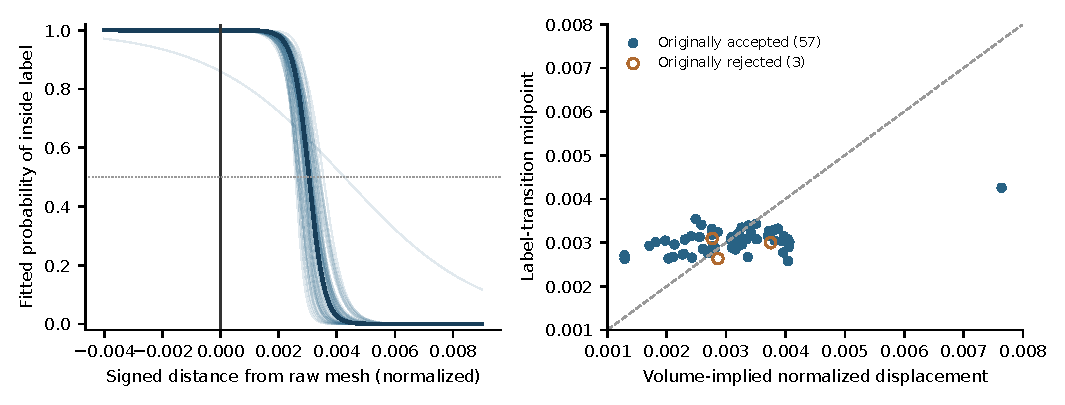
\includegraphics[width=\linewidth]{figures/boundary_verified.pdf}
\caption{Exact-distance boundary fits for the 57 objects accepted in the recorded analysis, replayed on the original queries. Left: object-specific fitted transitions (thin lines) and the transition at median fitted parameters (bold); zero marks the raw mesh. Right: label-transition midpoint versus volume-implied displacement, with identity line ($r=0.58$). Open markers show the three fits that failed the acceptance checks; they are excluded from the correlation.}
\label{fig:mechanism}
\end{figure*}

\subsection{The frozen correction transfers with reduced coverage}

Table~\ref{tab:IV} compares internal and frozen second-batch performance. The occupancy-only correction reduced internal MdAPE from 3.035\% to 0.580\%. On the 2,728 new objects, it reduced MdAPE from 3.481\% to 0.664\% and RMSE from 5.743\% to 1.743\%, reductions of 80.9\% and 69.7\%. Its second-batch mean signed bias was $+0.006$\% (95\% bootstrap interval $-0.059$\% to $+0.076$\%), and the MdAPE interval was 0.636\%--0.700\%.

\begin{table}[!t]
\caption{Correction performance. Errors are percentages relative to mesh volume. Coverage uses each method's own calibrated absolute-error bound.}
\label{tab:IV}
\centering
\footnotesize
\setlength{\tabcolsep}{2.5pt}
\renewcommand{\arraystretch}{1.15}
\begin{tabular}{@{}lrrrrr@{}}
\toprule
\textbf{Method} & \textbf{Bias} & \textbf{MdAPE} & \textbf{RMSE} & \textbf{Bound} & \textbf{Cov.} \\
\midrule
\multicolumn{6}{@{}l}{\textit{Internal test, n = 550}} \\
Uncorrected & $+3.608$ & 3.035 & 4.286 & 8.451 & 96.4\% \\
Global correction & $-0.040$ & 1.370 & 2.231 & 4.632 & 96.4\% \\
Occupancy-only & $-0.032$ & 0.580 & 1.149 & 2.661 & 96.2\% \\
\midrule
\multicolumn{6}{@{}l}{\textit{Frozen second batch, n = 2,728}} \\
Uncorrected & $+4.497$ & 3.481 & 5.743 & 8.451 & 90.0\% \\
Global correction & $+0.817$ & 1.503 & 3.542 & 4.632 & 90.0\% \\
Occupancy-only & $+0.006$ & 0.664 & 1.743 & 2.661 & 92.1\% \\
\bottomrule
\end{tabular}
\end{table}

A near-zero mean residual does not imply uniformly accurate estimates. Coverage of the occupancy-only bound fell to 92.1\% (bootstrap interval 91.1\%--93.0\%). Corrected second-batch pass rates at 2.17\%, 5\%, 6\%, and 10\% were 88.5\%, 98.0\%, 98.8\%, and 99.7\%. Fig.~\ref{fig:frozen} shows the complete absolute-error distributions, including the tails; the vertical line marks the occupancy-only bound. The uncorrected and global methods have identical coverage in both evaluations because they cover the same objects. The global correction divides every estimate by $k=1+c/100$, where $c=3.65$\% is the mean training error. It therefore covers raw errors from $c-b_gk=-1.15$\% to $c+b_gk=8.451$\%. The upper limit equals the uncorrected bound, because both calibration quantiles fall on the same calibration object, and no raw error fell below the lower limit.

\begin{figure}[!t]
\centering
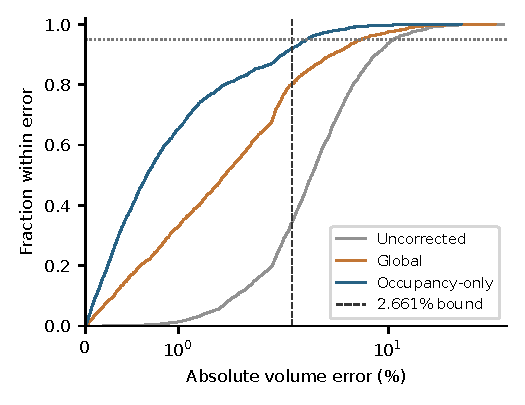
\includegraphics[width=\linewidth]{figures/frozen_ecdf.pdf}
\caption{Empirical cumulative distributions of absolute percentage error for all 2,728 second-batch objects. Every observation is included. The horizontal axis is linear near zero and logarithmic in the tail. The vertical line is the occupancy-only 2.661\% bound; the horizontal dotted line marks 95\% coverage.}
\label{fig:frozen}
\end{figure}

\subsection{The label pipeline reproduces the bias, and removing its depth offset removes about half of it}\label{sec:offsetres}

The reimplementation reproduced the released labels closely. At the default offset, a median of 98.0\% of sampled near-surface query points received the released label, compared with 91.7\% at offset 0 and 95.0\% at 0.75. Across objects, recreated and released volume errors were almost perfectly correlated (Pearson $r=0.999$), although the recreated errors were systematically smaller (median $+3.43$\% versus $+3.90$\%; median per-object difference 0.37 percentage points). In ten objects, replacing near-surface interpolated labels with mesh-containment labels (hybrid labeling) changed volume errors by at most 0.26 percentage points and did not close this gap; complete containment labeling was not tested.

Removing the depth offset lowered the occupancy-volume error in every one of the 55 objects, by a mean of 1.57 percentage points (95\% bootstrap interval 1.37--1.77), and the error rose monotonically across 0, 0.75, and 1.5 voxels (Fig.~\ref{fig:dose}, Table~\ref{tab:offset}). The fused-mesh volume error fell by 1.48 points, and in the 53 objects with accepted fits at both offsets the label midpoint moved inward in every object, by a mean of 0.00126. At zero offset a median error of $+1.58$\% remained. Removing the offset therefore removed about 45\% of the reproduced inflation. The source of the remainder was not isolated: depth-map erosion and truncated-distance fusion are candidate contributors, but neither was varied separately. The alternative coordinate convention and inclusion of the five pilot objects gave the same effect (1.59 and 1.58 points).

\begin{figure}[!t]
\centering
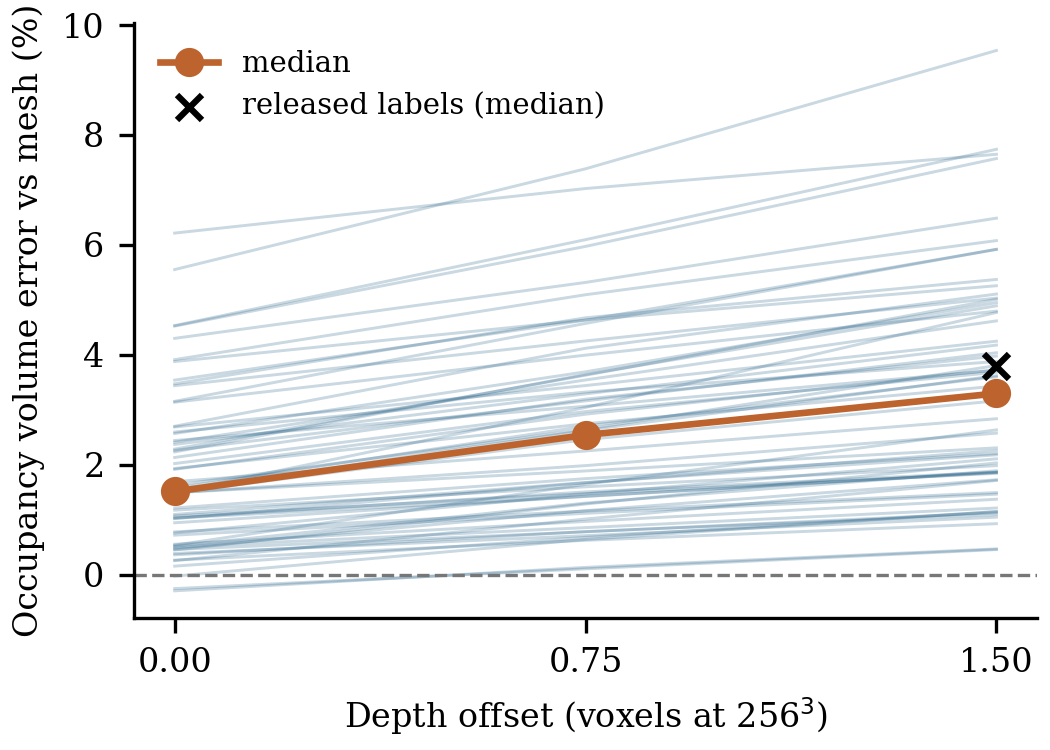
\includegraphics[width=\linewidth]{figures/offset_dose_response.png}
\caption{Controlled label-pipeline test (E8). Occupancy-volume error relative to the raw mesh at depth offsets of 0, 0.75, and 1.5 voxels; thin lines are individual objects and the cross marks the median error of the released labels. The plot includes the five pilot objects; statistics in the text use the other 55.}
\label{fig:dose}
\end{figure}

\begin{table}[t]
\centering
\caption{Controlled label-pipeline test ($n=55$). Signed occupancy-volume error relative to the raw mesh and agreement with the released labels.}
\label{tab:offset}
\footnotesize
\begin{tabular}{lrrr}
\toprule
Depth offset (voxels) & 0 & 0.75 & 1.5 \\
\midrule
Median error (\%) & 1.578 & 2.649 & 3.435 \\
Near-surface agreement (\%) & 91.7 & 95.0 & 98.0 \\
Accepted midpoint fits & 54/55 & 54/55 & 54/55 \\
\bottomrule
\end{tabular}
\end{table}

\subsection{Shape distribution and low occupancy define the transfer limits}

The second batch contained larger and less spherical objects: median sphericity was 0.793 versus 0.8358, median $A_m/V_m^{2/3}$ was 6.098 versus 5.786, and median occupancy fraction was 0.1138 versus 0.1437. Low-occupancy prevalence increased from 73/2,720 (2.7\%) to 181/2,728 (6.6\%).

Mean raw error increased by 0.833 percentage points. The development regression on shape complexity predicted an increase of 0.747 points, about 90\% of the observed change. The offset itself replicated: median volume-implied offsets were 0.00293 (development) and 0.00297 (second batch), with coefficients of variation of 0.28 and 0.27, and the slope of error on $A_m/V_m^{2/3}$ was 1.78 and 2.00 percentage points per unit ($R^2=0.67$ and 0.69). This descriptive decomposition associates most of the mean-error shift with changing shape complexity. The scale-aware predictor $A_ms/V_m$ fitted on development objects (slope 0.310, equivalent to $t_{\mathrm{norm}}=0.00310$) explained the second-batch errors without refitting ($R^2=0.83$; mean residual $-0.06$ points).

\begin{table*}[!t]
\caption{Occupancy-only coverage at the saved 2.661\% bound. Wilson intervals assume independent objects and do not quantify between-animal uncertainty.}
\label{tab:V}\centering\footnotesize
\setlength{\tabcolsep}{5pt}\renewcommand{\arraystretch}{1.15}
\begin{tabularx}{\textwidth}{Y Y r r r Y}
\toprule
\textbf{Evaluation} & \textbf{Group} & \textbf{Covered / total} & \textbf{Failures} & \textbf{MdAPE} & \textbf{Coverage [95\% interval]}\\
\midrule
Internal test & All & 529 / 550 & 21 & 0.580\% & 96.2\% [94.2, 97.5]\\
Internal test & Occupancy $<0.02$ & 7 / 16 & 9 & 3.011\% & 43.8\% [23.1, 66.8]\\
Internal test & Occupancy $\ge0.02$ & 522 / 534 & 12 & 0.551\% & 97.8\% [96.1, 98.7]\\
Second batch & All & 2,512 / 2,728 & 216 & 0.664\% & 92.1\% [91.0, 93.0]\\
Second batch & Occupancy $<0.02$ & 89 / 181 & 92 & 2.766\% & 49.2\% [42.0, 56.4]\\
Second batch & Occupancy $\ge0.02$ & 2,423 / 2,547 & 124 & 0.625\% & 95.1\% [94.2, 95.9]\\
\bottomrule\end{tabularx}\end{table*}

Table~\ref{tab:V} identifies much higher failure risk below occupancy 0.02, but the flag does not capture all violations: 124 of 216 second-batch failures (57.4\%) occurred outside it. Unflagged coverage decreased from 97.8\% internally to 95.1\% in the second batch. Reweighting the internal subgroup coverages to second-batch subgroup proportions gives 94.17\% coverage, versus 96.18\% internally and 92.08\% observed. This descriptive decomposition attributes 2.01 percentage points of the decline to subgroup composition and a further 2.09 points to within-group changes. The flag was defined in the initial audit, but using it as an applicability restriction is a later interpretation, and the observed 95.1\% is not a conditional guarantee. Within the second batch, coverage declined across shape-complexity deciles from 100\% to 64.1\%, and the highest decile remained under-corrected by a mean of $+1.45$\%. The worst 136 errors had median sphericity 0.557 and occupancy 0.017 (cohort medians: 0.793 and 0.114).

\subsection{Real EM processing preserves volume more than surface descriptors}

All 550 eligible MitoEM-R objects were meshed. The median mesh-versus-voxel volume difference was $-0.19$\% (5th--95th percentile $-0.35$\% to $-0.10$\%). The median mesh-versus-voxel-face surface difference was $-16.31$\%, illustrating the dependence of digitized-surface measurements on the area estimator \cite{ref30}. The median trimmed point-cloud extent difference was $-3.70$\%, whereas raw sampled extents differed by only $-0.03$\%, reproducing on real EM the trimming effect seen in 3DMSL.

\begin{table*}[!t]
\caption{MitoEM-R in-plane regridding relative to native-grid meshes for the same 550 objects. Brackets show 5th--95th percentiles.}
\label{tab:VI}
\centering
\footnotesize
\setlength{\tabcolsep}{4pt}
\renewcommand{\arraystretch}{1.15}
\begin{tabularx}{\textwidth}{Y Y Y Y Y}
\toprule
\textbf{Voxel spacing ($z\times y\times x$), nm} & \textbf{Volume change} & \textbf{Surface-area change} & \textbf{Sphericity change} & \textbf{Sphericity rank correlation} \\
\midrule
$30\times16\times16$ & +0.98\% [+0.45, +1.46] & $-5.84$\% [$-7.68$, $-4.72$] & +6.90\% [+5.68, +8.69] & 0.997 \\
$30\times24\times24$ & $-0.08$\% [$-0.93$, +0.41] & $-10.60$\% [$-12.14$, $-8.67$] & +11.76\% [+9.24, +13.75] & 0.994 \\
\bottomrule\end{tabularx}\end{table*}

All meshes in the original regridding analysis remained watertight. At the original 24 nm in-plane grid phase, volume rank correlation was 1.000 to reported precision, while median sphericity increased by 11.76\% (Table~\ref{tab:VI}). The near-zero volume change at 24 nm holds across grid alignments, but the 16 nm result does not: across all block phases and tie rules (S3, Appendix~\ref{app:phase}), median volume changes ranged from $-0.22$\% to $+0.01$\% at 24 nm but from $-5.47$\% to $+6.94$\% at 16 nm. Euler characteristics changed in nine of 550 objects at each spacing, so watertightness does not guarantee topology preservation. These shifts characterize this annotation-processing procedure; they are not correction factors for other tissues or instruments.



\section{Discussion}

\subsection{Measurement agreement is a prerequisite for biological interpretation}

The experiments separate three properties that are easily conflated. First, an estimator can be numerically precise while targeting a boundary that differs from the reference mesh: sampling SD was about 0.8\%, while the systematic offset was nearly four times larger. Second, a correction can remove average bias while leaving substantial errors in a morphological subgroup. Third, object rankings can remain stable while a descriptor's absolute scale changes. The high ICC, the near-zero corrected mean bias, and the high regridding rank correlations are each informative, but none alone establishes interchangeability.

For structure-function studies, a processing-induced change in sphericity could enter a classifier as though it were a cellular response, and rank preservation could hide a shifted absolute threshold. The findings give three practical recommendations for users of 3DMSL and similar resources. First, occupancy labels describe a surface about 0.003 normalized units outside the released mesh, so volumes computed from them, and models trained on them, inherit a bias whose relative size scales with $A_ms/V_m$. Second, in our reimplementation, regenerating labels with zero depth offset removed only about half of this bias; labeling query points directly against the released mesh avoids the fusion step altogether. Third, when occupancy-derived volumes must be used, a mesh-free correction reduces typical error about fivefold, but its uncertainty bound should not be relied on for objects with occupancy fraction below 0.02, and it does not guarantee coverage for other objects either.

\subsection{Correction transfer and uncertainty transfer are separate results}

The occupancy-only model performed well on typical second-batch objects and improved substantially on both raw volumes and a global correction. Observed coverage was near 95\% in the unflagged group and about 49\% in the flagged group. Coverage also declined within the unflagged group between evaluations, and aggregate subgroup coverage does not ensure coverage for every shape class. This pattern illustrates the distinction between marginal and conditional coverage \cite{ref29}. Conditional residual scales, Mondrian calibration by occupancy group, or covariate-shift weighting \cite{ref28} are natural next steps, but they require new development, and that batch could not serve as an untouched test for methods selected using its outcomes. The original correction and its reduced coverage are retained here as the primary transfer evidence.

\subsection{Implications for Homeostatic Invariance}

One potential application is Homeostatic Invariance, which we propose as a framework in which structural variability may coexist with maintained function within a bounded biological regime. The findings address a measurement prerequisite for testing that proposition; they do not test the proposition itself. A future biological stability region should distinguish structural variation that exceeds processing uncertainty from variation in independently measured function. That study would need aligned functional observations, longitudinal or perturbational designs, and replication across biological units. The present datasets contain no linked respiration, ATP, or membrane-potential measurements, so they cannot establish preserved function or a transition boundary.

\section{Limitations}

The two 3DMSL batches share dataset construction and upstream provenance; disjoint IDs do not establish independent acquisitions or animals, and source-object lineage and geometric equivalence were not resolved, despite no cross-batch identical mesh-file hashes. Object-level bootstrap intervals may be optimistic under spatial or biological dependence. The MitoEM-R analysis covers one rat-cortex volume and excludes boundary-truncated, small, shallow, and very large objects.

The internal split followed exploratory analysis, and E8 and the supplementary analyses were added after the primary results had been inspected (Appendix~\ref{app:history}). The boundary analysis and E8 use 60 objects from one batch. E8 is a reimplementation rather than the historical code, whose version has not been confirmed with the dataset authors; it under-predicts the released errors by a median of 0.37 percentage points, labels points from the interpolated field (checked only by a partial, near-surface containment replacement in ten objects), and does not separate the contributions of erosion and fusion. No new-source evaluation of the correction was performed. The regridding experiment leaves $z$ unchanged and does not model the point-spread function, segmentation uncertainty, or acquisition process of another instrument. Candidate tolerances were not prospectively established as biological equivalence margins.

\section{Conclusion}

Across 5,448 disjoint 3DMSL IDs, high representation agreement concealed a consistent positive occupancy-volume bias. A controlled reimplementation of the label pipeline reproduced the bias object by object, and setting the pipeline's depth offset to zero removed about half of it; the source of the remainder was not isolated. A mesh-free correction transferred to the second batch with an MdAPE of 0.664\%, but its uncertainty bound under-covered: 92.1\% overall, 49.2\% within a low-occupancy flag and 95.1\% outside it, with 124 of 216 failures outside the flag. In real EM, regridding preserved ranks while materially changing surface area and sphericity. Numerical precision, representation bias, uncertainty coverage, and descriptor scale should therefore be reported separately. These results provide a measurement foundation for studies that pair mitochondrial morphology with function.

\section*{Data and Code Availability}

3DMSL \cite{ref12} and MitoEM \cite{ref15} are publicly available. The accompanying reproducibility package contains the analysis code, executed notebooks, per-object tables, split identifiers, the frozen model (SHA-256 prefix 93b6daed) with its stored predictions and protocol, and all E8 and supplementary outputs, with a map from each reported result to its files. Applying the archived model to the archived descriptors reproduces every stored second-batch residual to within $7\times10^{-14}$ percentage points. The repository location is \url{\repourl}; upload of the accompanying package and creation of a versioned release are pending.

\section*{Ethics Statement}

This study analyzed only publicly available, previously published datasets. No new animal experiments or human-participant research were conducted.


\appendices
\section{Supplementary Imaging Analysis (S1)}

We tested whether 2D threshold morphometry of the released 3DMSL simulated microscopy images recovers object geometry. For 300 development objects sampled without replacement with seed 790, three configurations (Conf1 confocal, 70 nm pixels; Conf2 confocal, 48.8 nm; Epi1 widefield, 109 nm) and six orientations each, we segmented half-peak signal above a border-background estimate, applied morphological closing and hole filling, and retained the largest component. The analysis processed 1,798 Conf1 views and 1,800 views each for Conf2 and Epi1, with no empty or edge-touching masks. Image areas were compared with view-specific mesh silhouettes and sections that follow the simulator's centering and rotation; selection of the best-matching target was exploratory.

The results were negative. Geometry explained only 13\%--28\% of the orientation-to-orientation variation in image area. Cross-configuration ICC(A,1) for area was 0.509 for Conf1 versus Conf2, and 0.051 and 0.058 for the two Epi1 pairs; the corresponding rank correlations were 0.392, 0.344, and 0.631. Image-to-geometry area ratios were about 0.77 for the confocal configurations and 2.82 for Epi1. Rescaling the 109 nm Epi1 pixels to match the confocal ratio gives $109\sqrt{0.77/2.82}\approx57.0$ nm; matching unit image-to-geometry agreement instead gives $109/\sqrt{2.82}\approx64.9$ nm. These are diagnostic rescalings, not independently measured pixel calibrations. The supplied code notes a different pixel size in another repository widefield configuration, so simulator-configuration provenance remains unresolved. Blur, thresholding, focal geometry, and calibration can all contribute. All three configurations were noisy (median signal-to-noise ratio 6--18), and objects spanned only a few pixels near the optical resolution limit (124--245 nm). Bright hotspots caused the half-peak threshold to miss dimmer parts of objects, and an Otsu threshold captured background noise. For these simulated configurations and the tested half-peak and Otsu thresholds, image-derived areas did not reliably recover the candidate mesh targets. This finding does not establish a limitation of all segmentation methods or all optical acquisition conditions. These images were not used for the main analyses.

\section{Supplementary Correction-Model Comparison (S2)}

After the original outcomes had been inspected, we compared the retained five-feature ordinary least-squares (OLS) correction with occupancy-fraction-only OLS and with ridge regression on the same five features (Table~\ref{tab:model_sensitivity}). Each model used the saved development training split, and residual bounds used only the calibration split. Ridge used 36 log-spaced penalties from $10^{-3}$ to $10^4$, chosen by mean squared error over five unshuffled folds within training, with standardization refit inside each fold ($\alpha=0.251$). Refitting the retained model reproduced the stored second-batch residuals across all 2,728 objects to within $4.5\times10^{-14}$ percentage points. Compared with retained OLS, second-batch MdAPE was higher by 0.839 percentage points for the global correction (95\% paired object-bootstrap interval 0.782--0.889), 0.263 for fraction-only OLS (0.221--0.305), and 0.001 for ridge ($-0.003$ to 0.006). Occupancy fraction alone is therefore insufficient, and regularization does not change the result. This is not a formal equivalence test.

\begin{table}[t]
\centering
\caption{Exploratory second-batch model comparison ($n=2{,}728$). MdAPE and RMSE are percentages; coverage is the percentage within each model's own development-calibrated bound. Ridge uses corrected fold-specific scaling.}
\label{tab:model_sensitivity}
\begin{tabular}{lrrr}
\toprule
Correction & MdAPE & RMSE & Coverage (\%) \\
\midrule
None & 3.481 & 5.743 & 90.03 \\
Global mean & 1.503 & 3.542 & 90.03 \\
Occupancy fraction only & 0.927 & 2.718 & 89.37 \\
Retained five-feature OLS & 0.664 & 1.743 & 92.08 \\
Ridge, same features & 0.665 & 1.747 & 91.97 \\
\bottomrule
\end{tabular}
\end{table}

\section{Supplementary Grid-Phase Sensitivity (S3)}\label{app:phase}

The regridding of E7 was repeated for all four in-plane block phases at factor two, with ties assigned to foreground or background, and all nine phases at factor three: 17 configurations and 9,350 remeshed object/configuration pairs, all producing nonempty meshes (Fig.~\ref{fig:phase}). The original phase begins at the lower bound of each cropped object ROI. Foreground component counts use 6- and 26-neighbor connectivity, and Euler characteristics use 26-neighbor connectivity. At 16 nm, median volume changes ranged from $+0.58$\% to $+6.94$\% across phases with foreground ties and from $-5.47$\% to $+0.89$\% with background ties. At 24 nm they ranged from $-0.22$\% to $+0.01$\%. At the original phase, 26-neighbor component counts changed in one of 550 objects at each spacing.

\begin{figure*}[!t]
\centering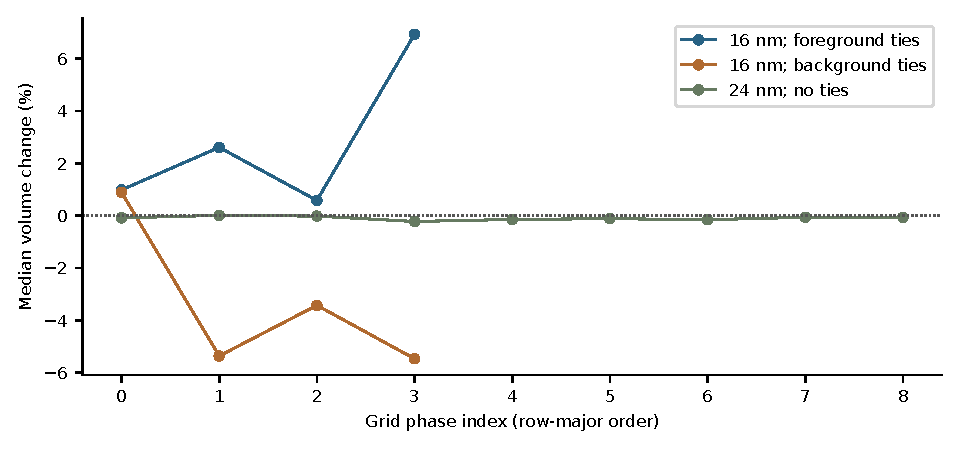
\includegraphics[width=0.62\linewidth]{figures/phase_sensitivity.pdf}
\caption{Exploratory grid-phase sensitivity for all 550 eligible MitoEM-R objects. Each point is the median volume change from its native-grid mesh. Phase indices enumerate $(y,x)$ offsets in row-major order, starting at $(0,0)$: four phases for factor two and nine for factor three. Leading zero padding changes the block origin without cropping the object. Lines connect the discrete phase configurations for readability.}
\label{fig:phase}\end{figure*}

\begin{figure*}[!t]
\centering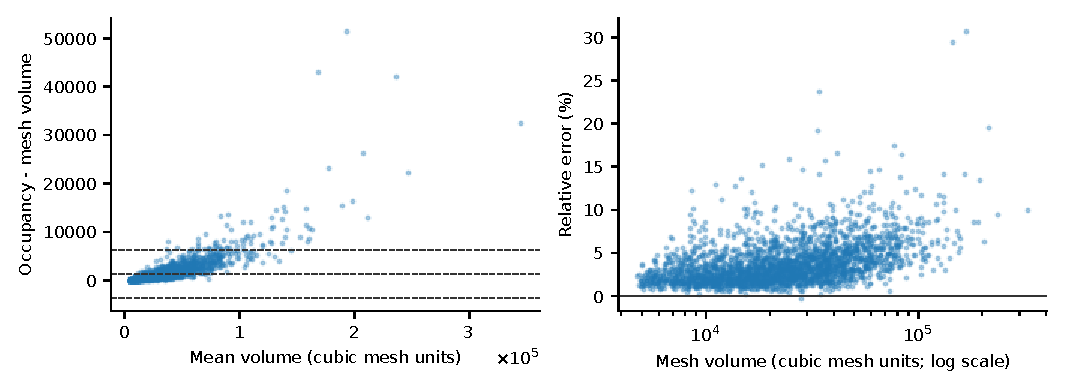
\includegraphics[width=0.72\linewidth]{figures/agreement_diagnostics.pdf}
\caption{Development-batch agreement diagnostics for all 2,720 objects. Left: absolute differences versus pair means, with pooled bias and limits of agreement. Right: relative errors versus mesh volume. The size-dependent pattern limits interpretation of pooled absolute limits as universal error bounds.}
\label{fig:agreement}\end{figure*}

\section{Analysis History and Deviations}\label{app:history}

This appendix records decisions made after the primary results, so that the main text can report what was done.

\emph{Low-occupancy flag.} The flag ($p<0.02$) was part of the quality-control policy applied in the initial audit; the QC output recording 73 flagged development objects (audit\_descriptors\_qc.csv) predates the development of the correction. Its later use as an applicability restriction is a post hoc interpretation.

\emph{Development and frozen evaluation.} Whole-batch exploration preceded the internal split, so the internal test is validation after exploration. The frozen second-batch evaluation used the archived model without refitting; all five protocol-listed input hashes match, and direct application of the archived model reproduces the stored residuals to within $7\times10^{-14}$ percentage points.

\emph{Boundary fits (E5).} Three of 60 fits failed the optimizer-success screen and are excluded from primary summaries. In a later replay all 60 converged; including them gives median $t_{50}=0.00304$ and $r=0.57$. The implied-offset correlation is sensitive to one object (25660): omitting it lowers Pearson $r$ from 0.577 to 0.312 and Spearman $\rho$ from 0.351 to 0.315. It was not excluded. The simple geometric expectation of half the depth shift ($0.5\times1.5/(256\times0.9)=0.00326$) is 1.07 times the measured midpoint, but E8 shows the depth offset alone moves the midpoint by only 0.00126, so this ratio should not be read as quantitative agreement.

\emph{Label-pipeline reimplementation (E8).} The first five of the 60 E5 objects (24558, 24611, 24853, 24898, 24925) were run as an engineering pilot and then, inadvertently, again in the full run; their results were identical. They were excluded from the primary analysis after the full results had been inspected; all 60 give a mean effect of 1.58 points (1.39--1.77). The repository code places marching-cubes vertices half a voxel from voxel centers, so labels were computed with and without this shift. The selection rule, higher agreement with the released labels, was written into the analysis script, whose SHA-256 hash (prefix 30b237e2) was recorded in the environment record at 16:12 UTC on 26 September 2026, before the pilot and full runs; the choice itself was made from the full-run results: the centered version agreed for 98.0\% of near-surface points and the shifted version for 90.2\%, and the offset effect was 1.57 and 1.59 points. Agreement is computed on up to 3,000 sampled near-boundary points per object. Midpoint fit-acceptance flags were saved without failure reasons, and acceptance for released-label fits was not saved. The hybrid containment check used the first ten non-pilot objects at offsets 0 and 1.5; winding-number containment replaced interpolated labels where the interpolated field was below $2/256$ in magnitude, and labels elsewhere were retained. In these objects the offset effect was 1.57 points with hybrid labels and 1.68 with interpolated labels. Complete containment labeling of every query point was not performed.

\emph{Model comparison (S2).} The first ridge run standardized the training set before cross-validation; the rerun fits standardization within folds. The selection criterion was also changed from mean fold $R^2$ to mean squared error, so the change in selected penalty ($0.398$ to $0.251$) should not be attributed to scaling alone. Displayed metrics changed by at most 0.03 percentage points.

\emph{Other checks.} Using the nominal query-box width $1.1s$ instead of the observed coordinate spans raises occupancy volume by a median 0.107\% in each batch and does not alter the retained estimator. The grid-phase checks (S3) and the scale-aware diagnostic were added after the audit and were not prospectively registered.

\bibliographystyle{IEEEtran}
\bibliography{references}
\end{document}
